\documentclass[11pt,a4paper]{report}
\usepackage[utf8]{inputenc}
\usepackage{amsmath}
\usepackage{amsfonts}
\usepackage{amssymb}
\usepackage{graphicx}
\usepackage{enumitem}
\usepackage[left=2cm, right=2cm, top=4.5cm, bottom=2cm]{geometry}
\usepackage{xstring}
\usepackage{tikz}
\usetikzlibrary{calc}



\begin{document}
	%Portada
	\begin{titlepage}
		\centering
		{\scshape\LARGE Universidad Nacional Autónoma de México \par}
		\vspace{1cm}
		{\scshape\Large Probabilidad I\par}
		\vspace{1.5cm}
		{\huge\bfseries Tarea Examen\par}
		\vspace{.5cm}

		{\Large\itshape Alan Ernesto Arteaga Vázquez \par}
		 \vspace{.5cm}
		{\Large\itshape Raúl Llamosas Alvarado \par}
		 \vspace{.5cm}
		{\Large\itshape Edgar Quiroz Castañeda \par}
	    \vspace{.5cm}
		{\Large\itshape Jean Paul Ruiz Melo\par}
		\vspace{.5cm}
		{\Large\itshape Sandra Del Mar Soto Corderi \par}

		\vfill
		 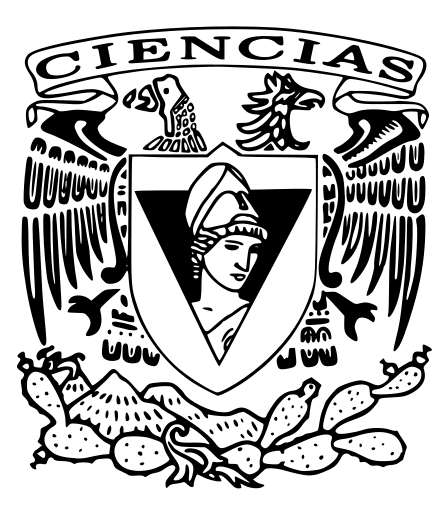
\includegraphics[width=0.3\textwidth]{escudo.png}
		\vfill

		{\large Lunes 3 de Diciembre del 2018 \par}
	\end{titlepage}

	\pagebreak
	\setlength{\voffset}{-0.75in}
	\setlength{\headsep}{5pt}

	%Ejericios
	\begin{enumerate}
		%1
		\item{
		\newcommand{\Size}{1cm}
        \def\NumOfColumns{5}
        \def\Sequence{1/A, 2/B, 3/C, 4/D, 5/E}
        \tikzset{Square/.style={
            inner sep=0pt,
            text width=\Size, 
            minimum size=\Size,
            draw=black,
            fill=white,
            align=center
            }
        }
        \newcommand{\NodeAA}{$\frac{y}{x}$}\newcommand{\NodeAB}{1}\newcommand{\NodeAC}{2}%
        \newcommand{\NodeAD}{3}\newcommand{\NodeAE}{4}%
        
        \newcommand{\NodeBA}{1}\newcommand{\NodeBB}{$(1,1)$}\newcommand{\NodeBC}{$(1,2)$}%
        \newcommand{\NodeBD}{$(1,3)$}\newcommand{\NodeBE}{$(1,4)$}%
        
        \newcommand{\NodeCA}{2}\newcommand{\NodeCB}{$(1,2)$}\newcommand{\NodeCC}{$(2,2)$}%
        \newcommand{\NodeCD}{$(2,3)$}\newcommand{\NodeCE}{$(2,4)$}%
        
        \newcommand{\NodeDA}{3}\newcommand{\NodeDB}{$(1,3)$}\newcommand{\NodeDC}{$(2,3)$}%
        \newcommand{\NodeDD}{$(3,3)$}\newcommand{\NodeDE}{$(3,4)$}%
        
        \newcommand{\NodeEA}{4}\newcommand{\NodeEB}{$(1,4)$}\newcommand{\NodeEC}{$(2,4)$}%
        \newcommand{\NodeED}{$(3,4)$}\newcommand{\NodeEE}{$(4,4)$}%
        
        \newcommand{\NodeFF}{$\frac{y}{x}$}\newcommand{\NodeFG}{1}\newcommand{\NodeFH}{2}%
        \newcommand{\NodeFI}{3}\newcommand{\NodeFJ}{4}\newcommand{\NodeFK}{$f_X(x)$}%
        
        \newcommand{\NodeGF}{1}\newcommand{\NodeGG}{$\frac{1}{16}$}\newcommand{\NodeGH}
        {$\frac{2}{16}$}\newcommand{\NodeGI}{$\frac{2}{16}$}\newcommand{\NodeGJ}
        {$\frac{2}{16}$} \newcommand{\NodeGK}{$\frac{7}{16}$}%
        
        \newcommand{\NodeHF}{2}\newcommand{\NodeHG}{0}\newcommand{\NodeHH}{$\frac{1}{16}$}%
        \newcommand{\NodeHI}{$\frac{2}{16}$}\newcommand{\NodeHJ}{$\frac{2}{16}$}%
        \newcommand{\NodeHK}{$\frac{5}{16}$}%
        
        \newcommand{\NodeIF}{3}\newcommand{\NodeIG}{0}\newcommand{\NodeIH}{0}%
        \newcommand{\NodeII}{$\frac{1}{16}$}\newcommand{\NodeIJ}{$\frac{2}{16}$}%
        \newcommand{\NodeIK}{$\frac{3}{16}$}%
        
        \newcommand{\NodeJF}{4}\newcommand{\NodeJG}{0}\newcommand{\NodeJH}{0}%
        \newcommand{\NodeJI}{0} \newcommand{\NodeJJ}{$\frac{1}{16}$}%
        \newcommand{\NodeJK}{$\frac{1}{16}$}%
        
        \newcommand{\NodeKF}{$f_Y(y)$}\newcommand{\NodeKG}{$\frac{1}{16}$}%
        \newcommand{\NodeKH}{$\frac{3}{16}$} \newcommand{\NodeKI}{$\frac{5}{16}$}%
        \newcommand{\NodeKJ}{$\frac{7}{16}$}%
        		
		Considere el experimento de lanzar dos tetraedros cuyos lados están numerados del 1 al 4. Sean $Y_{1},Y_{2}$ los números más pequeño y más grande obtenidos en las caras superiores respectivamente.\\
		Tenemos lo siguiente:
		\\
    	\centerline{
    	\begin{tikzpicture}[draw=black, ultra thick, x=\Size,y=\Size]
        \foreach \col/\colLetter in \Sequence {%
            \foreach \row/\rowLetter in \Sequence{%
                \pgfmathtruncatemacro{\value}{\col+\NumOfColumns*(\row-1)}
                \def\NodeText{\expandafter\csname Node\rowLetter\colLetter\endcsname}
                \node [Square] at ($(\col,-\row)-(0.5,0.5)$) {\NodeText};
                }
            }
        \end{tikzpicture}
        }
        
        \def\Sequence{1/F, 2/G, 3/H, 4/I, 5/J, 6/K}
		
		    
		    \begin{enumerate}
		        %(a)
		        \item {Encuentre la función de densidad conjunta de $Y_{1},Y_{2}$}\\
		        De esto se tiene:\\
		      \centerline{
    	            \begin{tikzpicture}[draw=black, ultra thick, x=\Size,y=\Size]
                         \foreach \col/\colLetter in \Sequence {%
                                \foreach \row/\rowLetter in \Sequence{%
                                    \pgfmathtruncatemacro{\value}{\col+6*(\row-1)}
                                    \def\NodeText{\expandafter\csname Node\rowLetter\colLetter\endcsname}
                                    \node [Square] at ($(\col,-\row)-(0.5,0.5)$) {\NodeText};
                                 }
                        }
                 \end{tikzpicture}
                }
			
		
		        %(b)
		        \item{Obtenga la densidad condicional de $Y_{2}$ dado $Y_{1}$ para cada uno de los posibles valores de $Y_{1}$}
		        \[ f(1|X) =\frac{P(X = x, Y = 1)}{P(X = x)} =
		        \frac{\frac{1}{16}}{\frac{7}{16}} + 
		        \frac{\frac{2}{16}}{\frac{7}{16}} +
		        \frac{\frac{2}{16}}{\frac{7}{16}} +
		        \frac{\frac{2}{16}}{\frac{7}{16}} =
		        .14 + .28 + .28 + .28\]
		        \[ f(2|X) =\frac{P(X = x, Y = 2)}{P(X = x)} =
		        \frac{0}{\frac{5}{16}} + 
		        \frac{\frac{1}{16}}{\frac{5}{16}} +
		        \frac{\frac{2}{16}}{\frac{5}{16}} +
		        \frac{\frac{2}{16}}{\frac{5}{16}} = 
		        .2 + .4 + .4\]
		        \[ f(3|X) =\frac{P(X = x, Y = 3)}{P(X = x)} =
		        \frac{0}{\frac{3}{16}} + 
		        \frac{0}{\frac{3}{16}} +
		        \frac{\frac{1}{16}}{\frac{3}{16}} +
		        \frac{\frac{2}{16}}{\frac{3}{16}} = 
		        .33 + .66\]
		        \[ f(4|X) =\frac{P(X = x, Y = 4)}{P(X = x)} =
		        \frac{0}{\frac{1}{16}} + 
		        \frac{0}{\frac{1}{16}} +
		        \frac{0}{\frac{1}{16}} +
		        \frac{\frac{1}{16}}{\frac{1}{16}} = 1\]
		        %(c)
		        \item{Encuentre $E(Y_{1}Y_{2}),E(Y_{1}),E(Y_{2})$}\\
		        \[E(Y_{1}Y_{2}) = E(XY) =
		        \frac{1}{16} + 2\frac{2}{16} +3\frac{2}{16} +4\frac{2}{16} + 
		       0 + (2\times2)\frac{1}{16} + (2\times3)\frac{2}{16} + (2\times4)\frac{2}{16} +\]
		        \[0 + 0 + (3\times3)\frac{1}{16} + (3\times4)\frac{2}{16} + 0 + 0 + 0 + (4\times4)\frac{1}{16}\]
		        \[= \frac{1}{16} + \frac{4}{16} + \frac{6}{16} + \frac{8}{16} + \frac{4}{16} + \frac{12}{16} + \frac{16}{16} +
			\frac{9}{16} + \frac{24}{16} + \frac{16}{16} = \frac{84}{16} = 5.25\]
		        \[E(Y_1) = E(X) = \frac{7}{16} + 2(\frac{5}{16}) + 3(\frac{3}{16}) + 4(\frac{1}{16}) = 1.875\]
		        \[E(Y_2) = E(Y) = \frac{1}{16} + 2(\frac{3}{16}) + 3(\frac{5}{16}) + 4(\frac{7}{16}) = 3.125\]
		        
		        %(d)
		        \item{¿Son $Y_{1} $ y $Y_{2}$ independientes?}\\
		        Tenemos que para que sea independiente se debe cumplir que:
		        \[f_{X,Y}(x,y) = f_X(x)f_Y(y)\]
		        Entonces si $x=1,y=1$, ya vimos que $f_{X,Y}(1,1) = \frac{1}{16}$ , $f_X(1) = \frac{7}{16}$ y $f_Y(1) = 
			\frac{1}{16}$, entonces:
		         \[f_{X,Y}(1,1) = \frac{1}{16} \neq \frac{7}{256} = \frac{7}{16}\frac{1}{16} = f_X(1)f_Y(1)\]
		         Por lo tanto $Y_1$ y $Y_2$ no son independientes.
		        
		    \end{enumerate}
          
            
		}

		%2
		\item{
		Suponga que X es una variable aleatoria con distribución $Bin(100,\frac{1}{5})$. Utilizando el teoerema de DeMoivre-
		Laplace, calcular $P(15\leq X \leq 25)$. \\
		Tenemos que DeMoivre-Laplace dice:
		\[X-Bin(n,p) =\frac{x-np}{\sqrt{np(1-p)}} = z = \frac{x - 100(\frac{1}{5})}{\sqrt{100(\frac{1}{5})(\frac{4}{5})}} =
		\frac{x - 20}{4}\]
		Para X-N(0,1), entonces:
		\[P(15 \leq X \leq 25) = \phi(\frac{25 - 20}{4}) - \phi(\frac{15 - 20}{4})  = 
		\phi(\frac{5}{4}) - \phi(\frac{-5}{4}) = \phi(\frac{5}{4}) - (1 - \phi(\frac{5}{4}))\]
		\[\phi(1.25) - 1 + \phi(1.25) = 2( ) - 1 = 2(.8944) - 1 = 1.7888 - 1 = .7888\]
		
		}

		%3
		\item{
            En una tarde soleada, Augusto lanza dos dados 2160 veces (él casi no tiene nada que hacer). Sea X el número de veces que 2 aparece en alguna de las caras. Encontrar la probabilidad de que X sea menor a 55.
		}

		%4
		\item{
			Sean $X_{1},...,X_{n}$ variables aleatorias independientes. Use la función generadora de momentos para encontrar la distribución de $\sum_{i=1}^{n}X_{i}$ en los siguientes casos:\\
			\begin{enumerate}
			    %(a)
			    \item {Si $\forall i \ \in \lbrace 1,..,n \rbrace \ X_{i} \sim Gamma(r,\lambda)$}
			    
			    %(b)
			    \item{Si $\forall i \ \in \lbrace 1,..,n \rbrace \ X_{i} \sim Gamma(r_{i},\lambda)$ }
			    %(c)
                \item{Si $\forall i \ \in \lbrace 1,..,n \rbrace \ X_{i} \sim exp(\lambda)$ }
                %(d)
                \item{Si $\forall i \ \in \lbrace 1,..,n \rbrace \ X_{i} \sim Geo(p)$ }
                %(e)
                \item{Si $\forall i \ \in \lbrace 1,..,n \rbrace \ X_{i} \sim BinNeg(r,p)$ }
                %(f)
                \item{Si $\forall i \ \in \lbrace 1,..,n \rbrace \ X_{i} \sim BinNeg(r_{i},p)$ }
                %(g)
                \item{Si $\forall i \ \in \lbrace 1,..,n \rbrace \ X_{i} \sim Poisson(\lambda)$ }
                %(h)
                \item{Si $\forall i \ \in \lbrace 1,..,n \rbrace \ X_{i} \sim Bin(n,p)$ }
                %(i)
                \item{Si $\forall i \ \in \lbrace 1,..,n \rbrace \ X_{i} \sim Bin(n_{i},p)$ }
                %(j)
                \item{Si $\forall i \ \in \lbrace 1,..,n \rbrace \ X_{i} \sim N(\mu,\sigma_{i}^2)$ }
			\end{enumerate}
		}

		%5 
		\item{
		Sea $S_{n}$ el número de éxitos en n ensayos Bernouilli independientes. Demuestre que $$P(|\frac{S_{n}}{n}-p|\geq \epsilon)\leq \frac{1}{4n\epsilon^2}$$
			
		}

		%6
		\item{
		Sea S el número de águilas en 1,000,000 lanzamientos de una moneda honesta. Use (a) la desigualdad de Chebyshev y (b) el Teorema del Límite Central para estimar la probabilidad de que S esté entre 499,500 y 500,500.
		}

		%7
		\item{
			
          Si $X \sim Gamma(n,1)$ aproximadamente que tan grande debe ser n para que 
          $$P[|\frac{X}{n}-1|\geq 0.001]\leq 0.001$$
		}

		%8
		\item{
			Sean $X_{1},...,X_{20}$ variables aleatorias independientes tales que $\forall i \ \in \lbrace 1,...,20 \rbrace \ X_{i} \sim Poisson(\lambda) $ con media 1.\\
			\begin{enumerate}
			    %(a)
			    \item{Utilice la desigualdad de Markov para obtener una cota para $P[\sum_{i=1}^{20}X_{i}>15]$} 
			    %(b)
			    \item{Utilice el Teorema del Limite Central para aproximar $P[\sum_{i=1}^{20}X_{i}>15]$}
			\end{enumerate}
		}

		%9
		\item{
	    Sea $\lbrace X_{i} \rbrace _{i=1}^{\infty}$ una sucesión de variables aleatorias independientes. Suponga que $E(X_{i})=0$ y $Var(X_{i})=\sigma_{i}^{2}$ y suponga también que:
	            $$\lim_{n \rightarrow \infty}\sum_{i=1}^{n}\frac{\sigma_{i}^{2}}{n^2}=0$$
	   Demuestre que para cualquier $\epsilon >0$
	                $$P(\frac{|\sum_{i=1}^{n}X_{i}|}{n}>\epsilon)\rightarrow 0$$
	   Cuando $n\rightarrow \infty$.\\
	   Use lo anterior para probar que si $\lbrace Y_{i} \rbrace_{i=1}^{\infty}$ son variables aleatorias independientes tales que $Y_{i}\sim Bnnlli(p_{i})$ entonces para cualquier $\epsilon>0$, 
	                $$P(|\frac{\sum_{i=1}^{n}Y_{i}}{n}-p(n)|\leq \epsilon)\rightarrow 1$$
	   Cuando $n\rightarrow \infty$ donde $p(n)=\frac{\sum_{i=1}^{n}p_{i}}{n}$
		}

		%10
		\item{
			Explique por qué una variable aleatoria con distribución $Gamma(r,\lambda)$ tiene aproximadamente una distribución normal cuando r es grande. 
		}

		
	\end{enumerate}
\end{document}
